\chapter{Introduction}
  \section{What is \Kieker?}
    \Kieker\ is a framework which allows for example the monitoring and analysis of control flows, response times and runtime behavior of Java applications. Normal (``plain'') Java applications can be arranged with the framework as well as server based java web applications. The framework itself aims to provide an easy managable and maintanable piece of software, which can be included uncomplicated into existing software projects. \Kieker\ ist designed for a continous operation, resulting in a very small overhead during the monitoring. \Kieker\ can put whole method calls on a watch, but single statements (e.g. a = a + 1) as well.\\
    Nearly every component of the framework can be extended and adjusted easily as necessary.
    % This is the diagram which shows the single parts of Kieker as one component diagram (the 'satellite').
    \begin{figure}[H]
      \begin{center}
	\includegraphics[width=1.0\textwidth]{./images/kiekerComponentDiagram.pdf}
	\caption{The component diagram of \Kieker}
	\label{image:kiekercomponentdiagram}
      \end{center}
    \end{figure}
    As can be seen in Figure \ref{image:kiekercomponentdiagram}, the framework consists mainly of two big parts:
    \begin{itemize}
      \item \textbf{\KiekerMonitoring}\\
	This is the part which is responsible for the logging and the recording of the program behavior. The result of this component are the recorded informations which can then be written into different monitoring logs, like for example into files or into a database.
      \item \textbf{\KiekerAnalysis}\\
	This part is responsible for the evaluation and visualization of the recorded information. It uses the files (or general any collected data which is available as monitoring records) for the analysis and to produce graphs (e.g. Component-Dependency-Graph).
    \end{itemize}
    Both parts are composed of subcomponents which can be used or extended as well with own classes. The rough interaction between the different components is described by Figure \ref{image:interactiondiagramofkieker} but will be explained furthermore in the course of this tutorial.
    % This is the diagram which shows the interaction between the components and when which component get what kind of input.
    \begin{figure}[H]
      \begin{center}
	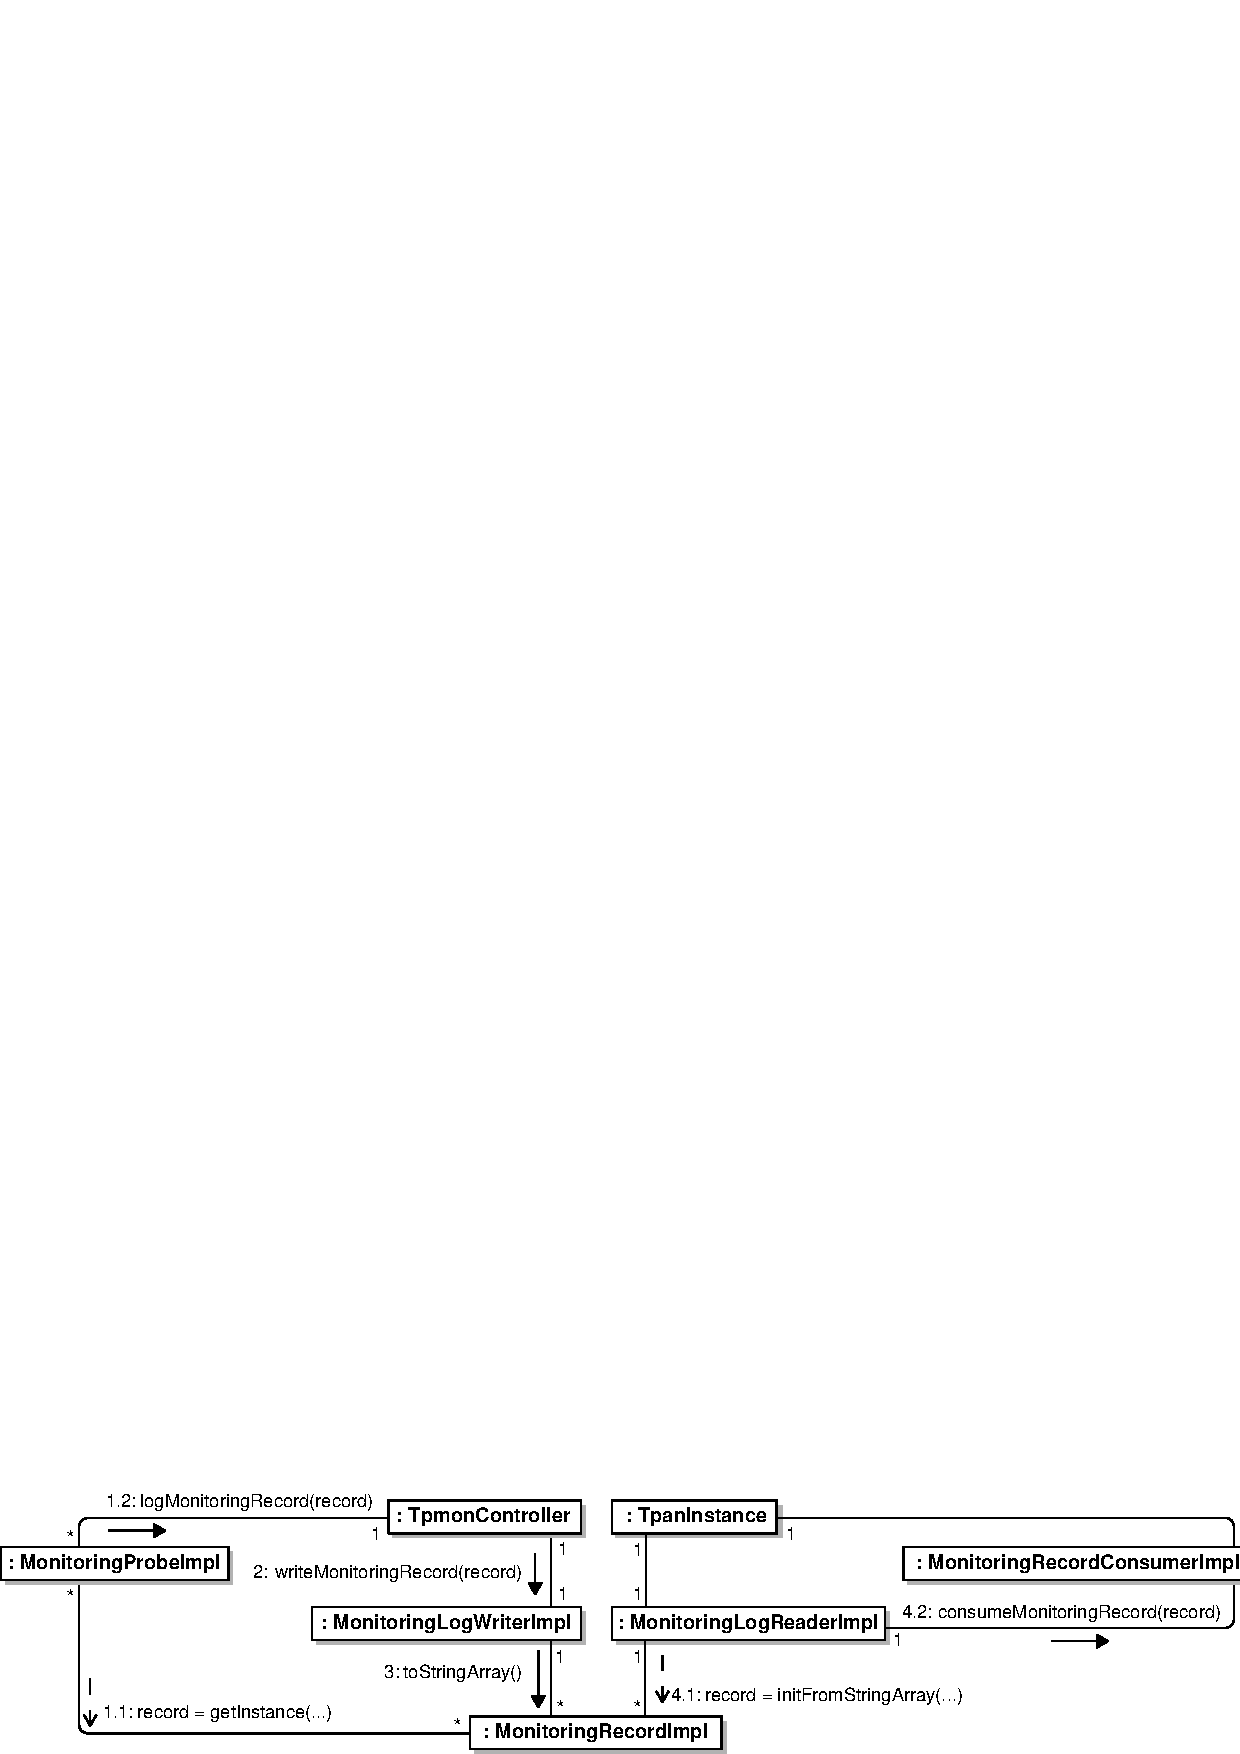
\includegraphics[width=1.0\textwidth]{./images/kiekerCommunications-revisedReArranged-woMonitoringLog-bw.pdf}
	\caption{Interaction between the components of \Kieker}
	\label{image:interactiondiagramofkieker}
      \end{center}
    \end{figure}
    The monitoring probes create either the monitoring records manually or by calling the monitoring controller. The monitoring controller uses the monitoring log writers to persist the given records which can then be later read by a monitoring log reader who creates a monitoring record again. This monitoring records can then be used by the consumer in nearly every way.

  \section{Features}

  \section{What ist the purpose of this tutorial?}
    In this tutorial, we will take a closer look at both, the \textbf{\KiekerMonitoring}- and the \textbf{\KiekerAnalysis}-part. That means, we will describe on the one hand how \KiekerMonitoring\ can be used to mark parts of the own sourcecode for \Kieker\ and to let them execute under surveilance, so that the recorded information can be saved somewhere and on the other hand we will use \KiekerAnalysis\ to process (for example visualize) our recorded data.\\
    We will show how to create and execute a simple example before we go deeper into the single parts of the framework.